\section{Small witnesses for four and five classical colors}\label{sec:finite}

For the first level of the square substitution, $S_\lambda(K_3)$ of Theorem~\ref{thm:one-level} has $342+81\lambda$ vertices: six basis charts of $57$ words plus $\lambda$ interior layers of $9$ vertices on each of the nine wires. When only $1$-compatibility is required, substantially smaller graphs already witness the first two gaps $(\cq,\chi)=(3,4)$ and $(\cq,\chi)=(3,5)$. In this section we exhibit the smallest known explicit witnesses for these gaps---graphs on $22$ and $165$ vertices---determine which of them can serve as a starting graph for the iterated substitution, and lift Lalonde's $15$-vertex lower bound on $N_3(4,1)$ to a new lower bound $N_3(5,1)\ge21$.

\subsection{Four classical colors on \texorpdfstring{$22$}{22} vertices}\label{sec:f22}

\begin{proposition}\label{prop:twentytwo}
There is a graph $F_{22}$ on $22$ vertices and $42$ edges with $\cq=3$ and $\chi=4$. Every quantum $3$-coloring of $F_{22}$ has local dimension divisible by four, and there is one in local dimension four.
\end{proposition}
\begin{proof}
Construct $F_{22}$ as follows. Take a \emph{center} vertex $o$ adjacent to nine \emph{terminals} $A,\bar A,B,\bar B,C,\bar C,X,Y,Z$, and add the three edges $A\bar A$, $B\bar B$, and $C\bar C$ joining each barred terminal to its unbarred partner. For each of the six entries in the table below, introduce a new \emph{private edge} $uv$, joining $u$ to the indicated left pair of terminals and $v$ to the indicated right pair:
\[
\begin{array}{cc|cc|cc}
\text{left}&\text{right}&\text{left}&\text{right}&\text{left}&\text{right}\\ \hline
 A,X&Z,\bar C & X,B&Y,\bar C & A,Y&B,Z\\
 \bar A,X&C,Z & X,\bar B&Y,C & \bar A,Y&\bar B,Z
\end{array}
\]
This yields $1+9+12=22$ vertices and $9+3+6\cdot5=42$ edges.

\emph{Classical chromatic number $\chi(F_{22})=4$.} Suppose $F_{22}$ had a proper classical $3$-coloring. Because all nine terminals are adjacent to $o$, they use only the two colors different from the color of $o$; encode those two colors as bits in $\{0,1\}$. Since $A\bar A,B\bar B,C\bar C$ are edges, each barred terminal carries the complement of its partner's bit. On any private edge $uv$, if both $u$ and $v$ saw unequal terminal bits on their attached pairs, then both $u$ and $v$ would be forced to take the color of $o$, violating the edge $uv$. Thus every private edge forbids simultaneous disagreement on its left and right pairs. Checking the two rows in the first column pair of the table: if $A=X$ (so $\bar A\ne X$), the second row forces $C=Z$; if $A\ne X$, the first row forces $Z=\bar C$, i.e., $C\ne Z$. Together these give $A\oplus X=C\oplus Z$. By the same check on the second and third column pairs,
\[
 A\oplus X=C\oplus Z,\qquad X\oplus B=Y\oplus C,\qquad A\oplus Y=1\oplus B\oplus Z.
\]
Summing all three equations modulo $2$ cancels every terminal bit and yields $0=1$, a contradiction. Conversely, $4$ colors suffice: color the unbarred terminals with color $1$, the barred terminals with color $2$, the center $o$ and all left private endpoints $u$ with color $3$, and all right private endpoints $v$ with color $4$. Hence $\chi(F_{22})=4$.

\emph{Quantum $3$-coloring in local dimension four.} Write $x,y,z$ in lower case for the single-qubit Pauli matrices (to distinguish them from the terminals $X,Y,Z$). Assign to the six unbarred terminals the two-qubit observables
\[
\begin{array}{lll}
 A=I\otimes z,& B=x\otimes x,& C=z\otimes x,\\
 X=x\otimes I,& Y=z\otimes I,& Z=y\otimes y,
\end{array}
\]
and assign to each barred terminal $\bar S$ the negated observable $-S$. The two observables in every left or right pair of the table commute, and they satisfy the hexagon relations
\[
 AX=CZ,\qquad XB=YC,\qquad AY=-BZ
\]
(Figure~\ref{fig:hexagon}). Color the center $o$ deterministically with outcome $0$ ($P_{o,0}=I$). At each terminal with observable $S$, return outcome $1$ on its $+1$ eigenspace $(I+S)/2$ and outcome $2$ on its $-1$ eigenspace $(I-S)/2$. At each private-edge endpoint attached to commuting terminal observables $U,V$, assign outcomes $0,1,2$ to the three pairwise orthogonal projectors
\[
 \frac{I-UV}{2},\qquad \frac{(I-U)(I-V)}{4},\qquad \frac{(I+U)(I+V)}{4},
\]
which sum to $I$. Outcome $1$ lies inside the $-1$ eigenspaces of both $U$ and $V$ (avoiding their outcome $1$), and outcome $2$ lies inside the $+1$ eigenspaces of both $U$ and $V$ (avoiding their outcome $2$), satisfying all terminal-to-endpoint edges. Across every private edge $uv$, write $U,V$ for the two terminal observables attached to $u$ and $U',V'$ for those attached to $v$. The products $UV$ and $U'V'$ are negatives of each other, by the hexagon relations and the signs of the barred terminals. Thus the outcome-$0$ projectors $(I-UV)/2$ at $u$ and $(I-U'V')/2=(I+UV)/2$ at $v$ are orthogonal. The projectors of the outcomes $1$ and $2$ lie in the range of $(I+UV)/2$ at $u$ and in the range of $(I-UV)/2$ at $v$, so they are orthogonal as well. Every edge rule therefore holds.

The vertices $o,A,\bar A$ form a triangle, so $\cq(F_{22})=3$. Finally, Proposition~\ref{prop:small-dimension} in Appendix~\ref{app:small-dimension} proves that every finite-dimensional quantum $3$-coloring of $F_{22}$ has local dimension divisible by four.
\end{proof}

\begin{figure}[htbp]
\centering
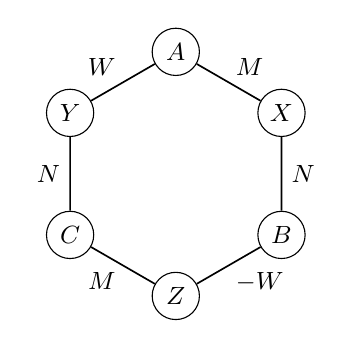
\begin{tikzpicture}[x=1cm,y=1cm,
   point/.style={circle,draw=black,fill=white,inner sep=1.5pt,minimum size=6mm,font=\small},
   every node/.style={font=\small}]
\foreach \name/\angle in {A/90,X/30,B/-30,Z/-90,C/-150,Y/150}
  \node[point] (\name) at (\angle:1.55) {$\name$};
\draw[semithick] (A) -- node[above right=-1pt] {$M$} (X) -- node[right] {$N$} (B)
 -- node[below right=-1pt] {$-W$} (Z) -- node[below left=-1pt] {$M$} (C)
 -- node[left] {$N$} (Y) -- node[above left=-1pt] {$W$} (A);
\end{tikzpicture}
\caption{The six tested pairs of terminals in $F_{22}$ form the edges of a hexagon. In the two-qubit strategy of Proposition~\ref{prop:twentytwo}, each edge carries the product of its two commuting observables, with $M=AX=CZ$, $N=XB=YC$, and $W=AY=-BZ$. No assignment of signs $\pm1$ to the six terminals satisfies these three relations. The six edge values would multiply to $+1$, because every terminal lies on two edges; but the relations give them the form $\varepsilon_1,\varepsilon_2,-\varepsilon_3,\varepsilon_1,\varepsilon_2,\varepsilon_3$ with $\varepsilon_1,\varepsilon_2,\varepsilon_3\in\{\pm1\}$, whose product is $-1$.}
\label{fig:hexagon}
\end{figure}

\subsection{Five classical colors on \texorpdfstring{$165$}{165} measurements}\label{sec:165}

We now trim the physical graph of $S_0(K_3)$ down to $165$ projective measurements that still require five classical colors and still carry a tower of length one. Identify the three colors with $C=\mathbb Z/3$. Call the positions $1,2,3$ of a basis of the square its \emph{tail positions}, and index them by $i\in C$ in order. In each of the six bases, retain the words
\begin{equation}\label{eq:finite-words}
 (k,\,k+p_0,\,k+p_1,\,k+p_2),\qquad
 k\in C,\quad
 p\in\{O,\alpha_i,\beta_i,\delta_i,\upsilon_i:i\in C\},
\end{equation}
where $O=(0,0,0)$, $\alpha_i=\mathbf 1-e_i$ (having $0$ in coordinate $i$ and $1$ in the other two coordinates), $\beta_i=-\alpha_i$, $\delta_i=-e_i$, and $(\upsilon_i)_s=s-i$ for $s\in C$. Notice that each of the $13$ difference triples $p$ has at least one zero coordinate, so every retained word repeats its first letter $k$ and belongs to the $57$ words of Section~\ref{sec:example}; there are $3\cdot13=39$ words per basis.

Assign to each word the three-outcome projective measurement in its basis that maps each ray to its indicated color, and identify equal measurements across bases:
\begin{itemize}
\item For $p=O$, all six bases share the $3$ constant measurements, which we call \emph{scalar} (matching the scalar projectors of Section~\ref{sec:substitution}).
\item For $p\in\{\alpha_i,\beta_i:i\in C\}$, each word takes one color on a shared plane $P_e$ and a second color on $I-P_e$, giving $6$ nonconstant measurements on each of the $9$ planes of~\eqref{eq:planes} ($9\cdot6=54$ measurements).
\item For $p\in\{\delta_i,\upsilon_i:i\in C\}$, each word has a color that occurs at a single ray (a rank-one outcome); because all $24$ basis rays of the square are distinct, these contribute $6\cdot(3\cdot6)=108$ distinct measurements.
\end{itemize}
In total, \eqref{eq:finite-words} yields $3+54+108=165$ distinct projective measurements on $\C^4$. Let $F_{\rm phys}$ be the physical graph on these $165$ measurements, joining two measurements $M,N$ whenever $M_aN_a=0$ for all $a\in C$. Its edge count is $843$ (computed by \texttt{checks/check\_square\_graphs.py}).

\begin{theorem}\label{thm:finite-square}
The graph $F_{\rm phys}$ satisfies $(\cq,\chi)=(3,5)$. There is a tower of length one over $F_{\rm phys}$, so that $w^3\ne0$ on its box complex. The graph has a quantum $3$-coloring in local dimension four and none in a smaller local dimension.
\end{theorem}
\begin{proof}
Appendix~\ref{app:finite} constructs an explicit tower of length one over $F_{\rm phys}$. Applying Proposition~\ref{prop:tower-bound} with $h=1$ immediately gives $w^3\ne0$ on $\B(F_{\rm phys})$ and $\chi(F_{\rm phys})\ge5$. Because $F_{\rm phys}$ is a subgraph of the physical graph of all three-label measurements in the six bases, Proposition~\ref{prop:physical-upper} in Appendix~\ref{app:five-coloring} (with $n=3$) gives $\chi(F_{\rm phys})\le5$; hence $\chi(F_{\rm phys})=5$.

Assigning each vertex of $F_{\rm phys}$ to its own projective measurement gives a quantum $3$-coloring in local dimension four, and the three scalar measurements form a triangle, so $\cq(F_{\rm phys})=3$. Finally, because $w^3\ne0$ implies $w^2\ne0$, Proposition~\ref{prop:height-dimension} excludes every odd local dimension (in particular $d=1$ and $d=3$), while Theorem~\ref{thm:qutrit}(a) excludes local dimension $d=2$ since $\chi(F_{\rm phys})>3$. Thus $F_{\rm phys}$ admits no quantum $3$-coloring in local dimension less than four.
\end{proof}

\subsection{Starting graphs for the iteration}\label{sec:no-seed}

Because $F_{\rm phys}$ carries a tower of length one, it can serve as a starting graph for the square substitution, saving one iteration relative to starting from $K_3$.

\begin{corollary}\label{cor:seed}
For all $j\ge1$ and $\lambda\ge0$, the graph $S^{j-1}_\lambda(F_{\rm phys})$ has quantum chromatic number three, with a quantum $3$-coloring in local dimension $4^j$, and classical chromatic number at least $2j+3$.
\end{corollary}
\begin{proof}
Applying Theorem~\ref{thm:step} with $h=1$ to the tower of length one over $F_{\rm phys}$ from Theorem~\ref{thm:finite-square} gives $\chi(S^{j-1}_\lambda(F_{\rm phys}))\ge 2(1+(j-1))+3=2j+3$. Starting from the identity quantum $3$-coloring of $F_{\rm phys}$ in local dimension four and applying~\eqref{eq:strategy} $j-1$ times produces a quantum $3$-coloring of $S^{j-1}_\lambda(F_{\rm phys})$ in local dimension $4^j$. The constant words on the three scalar measurements form a triangle at every level, so $\cq(S^{j-1}_\lambda(F_{\rm phys}))=3$.
\end{proof}

Corollary~\ref{cor:seed} claims no compatibility beyond the edge rule and no bound on the order. By contrast, a graph with $\chi=4$ can never carry a tower of length one, because Proposition~\ref{prop:tower-bound} forces $w^3\ne0$ and $\chi\ge5$. For $F_{22}$, even $w^2$ vanishes on $\B(F_{22})$.

\begin{proposition}\label{prop:no-seed}
There is an equivariant map from $\B(F_{22})$ to the circle $S^1$ with the antipodal involution. Consequently $w^2=0$ on the box complex of $F_{22}$, there is no tower of length one over $F_{22}$, and the bound~\eqref{eq:classical-obstruction} certifies only three of its four colors.
\end{proposition}
\begin{proof}
Use the proper $4$-coloring of $F_{22}$ from Proposition~\ref{prop:twentytwo}: color $1$ on unbarred terminals, color $2$ on barred terminals, color $3$ on the center $o$ and every left endpoint $u$ of a private edge, and color $4$ on every right endpoint $v$ of a private edge. For any point $(\mu,\nu)\in\B(F_{22})$, let $x\in\R^4$ be the color-mass difference vector whose entry $x_c$ equals the $\mu$-mass minus the $\nu$-mass of color class $c$, and define the continuous odd map $\varphi:\B(F_{22})\to\R^2$ by
\[
 \varphi(\mu,\nu)=(x_1-x_3,\;x_2-x_4).
\]
We claim that $\varphi$ never vanishes on $\B(F_{22})$.

Suppose for contradiction that $\varphi(\mu,\nu)=0$. Then $x_1=x_3$ and $x_2=x_4$. Since $\sum_{c=1}^4 x_c=1-1=0$, we also have $x_1+x_2=0$, so $x_1=x_3=-x_2=-x_4$. Because the coloring is proper and opposite shores are completely adjacent, the supports of $\mu$ and $\nu$ receive disjoint sets of colors; hence the positive and negative parts of $x$ have disjoint supports, each summing to $1$. Thus $x_1=x_3$ cannot vanish, and after swapping $\mu$ and $\nu$ if necessary we have $x_1=x_3=1/2$ and $x_2=x_4=-1/2$. In particular, $\operatorname{supp}\mu$ meets both color class $1$ and color class $3$, while $\operatorname{supp}\nu$ meets both color class $2$ and color class $4$.

Pick a barred terminal $\bar S\in\operatorname{supp}\nu$ (color $2$) and a right private endpoint $v\in\operatorname{supp}\nu$ (color $4$). Every vertex of $\operatorname{supp}\mu$ must be adjacent to both $\bar S$ and $v$:
\begin{itemize}
\item Pick an unbarred terminal $S'\in\operatorname{supp}\mu$ (color $1$). Because $S'$ is adjacent to $\bar S$, and the only unbarred terminal adjacent to $\bar S$ is its partner $S$, we must have $S'=S$. Complete adjacency to $v$ then implies that $S$ is attached to $v$.
\item Pick a vertex $q\in\operatorname{supp}\mu$ of color $3$. Because $o$ has no private-edge neighbor whereas $q$ is adjacent to $v$, $q$ must be the unique left endpoint $u$ of the private edge $uv$. Complete adjacency to $\bar S$ then implies that $\bar S$ is attached to $u$.
\end{itemize}
Thus $u$ is attached to $\bar S$ and $v$ is attached to $S$ on the same private edge $uv$. Inspection of the six rows of the table in Proposition~\ref{prop:twentytwo} shows that no private edge has a terminal on one side and its barred partner on the other. This contradiction proves $\varphi(\mu,\nu)\ne0$ everywhere on $\B(F_{22})$.

Normalizing gives the continuous equivariant map $\varphi/\|\varphi\|:\B(F_{22})\to S^1$. Pulling back from the quotient $\mathbb{RP}^1$ gives $w^2=0$ on $\B(F_{22})$ because $H^2(\mathbb{RP}^1;\Ftwo)=0$. For any space $Z$ mapping equivariantly to $\B(F_{22})$, $w_Z$ is a pullback of $w$, so $w_Z^2=0$, meaning~\eqref{eq:classical-obstruction} applies only for $k\le1$ ($\chi\ge3$). A tower of length one over $F_{22}$ would give $w_Z^3\ne0$ by Lemma~\ref{lem:tower-detection}, so none exists.
\end{proof}

\subsection{Lower bounds on the minimum order}\label{sec:small-lower}

The next proposition records Lalonde's $15$-vertex lower bound for graphs with a quantum $3$-coloring and $\chi\ge4$, and lifts it analytically to a new $21$-vertex lower bound for $\chi\ge5$, isolating the paper's sole reliance on an imported computer-assisted theorem.

\begin{proposition}\label{prop:order-lower}
Let $G$ be a graph with a quantum $3$-coloring. If $\chi(G)\ge4$, then $|V(G)|\ge15$. If $\chi(G)\ge5$, then $|V(G)|\ge21$. Consequently
\[
 15\le N_3(4,1)\le22,\qquad 21\le N_3(5,1)\le165.
\]
\end{proposition}
\begin{proof}
The single external input not proved in this article is Lalonde's computer-assisted classification~\cite[Theorem~1.1 of the arXiv version]{La}: every graph with $\cq<\chi$ has at least $15$ vertices, or has exactly $14$ vertices and $\cq\ge4$. We invoke this theorem exclusively in the following equivalent consequence for $\cq\le3$:
\begin{itemize}
\item[\textup{(L)}] Every graph on at most $14$ vertices that admits a quantum $3$-coloring is classically $3$-colorable.
\end{itemize}
Statement~(L) immediately yields the first claim: if $\chi(G)\ge4$, then $|V(G)|\ge15$. Because a quantum $3$-coloring restricts to every induced subgraph, (L) applies to every induced subgraph of $G$ on at most $14$ vertices.

Now suppose $\chi(G)\ge5$ and set $n=|V(G)|$. By~(L), $n\ge15$. Choose any $14$ vertices of $G$; by~(L), they induce a $3$-colorable subgraph, whose largest color class is an independent set $I$ of size at least $\lceil14/3\rceil=5$. Deleting $I$ leaves a graph $G-I$ that still admits a quantum $3$-coloring and requires at least $4$ classical colors, so $|V(G-I)|\ge15$ by~(L). Hence $n\ge 5+15=20$.

Suppose for contradiction that $n=20$. We reach a contradiction in five steps:
\begin{enumerate}
\item \emph{No independent set has size $6$.} Removing an independent set of size $6$ would leave a $14$-vertex induced subgraph requiring at least $4$ colors, contradicting~(L).
\item \emph{Every vertex has degree at least $7$.} If a vertex $v$ had at most $6$ neighbors, it would have at least $13$ non-neighbors; by~(L), those $13$ non-neighbors induce a $3$-colorable subgraph and hence contain an independent set of size $\lceil13/3\rceil=5$. Adjoining $v$ would produce an independent set of size $6$, contradicting Step~1.
\item \emph{No edge lies in two triangles.} Suppose $uvx$ and $uvy$ are triangles in $G$ with $x\ne y$. By the triangle identity (Fact~6 of Section~\ref{sec:coord-proj}), the three projectors for any fixed color $a$ on a triangle sum to $I$, so $P_{x,a}=I-P_{u,a}-P_{v,a}=P_{y,a}$ for all $a$. Thus $x$ and $y$ carry identical measurements and cannot be adjacent (by the edge rule). Identifying $x$ and $y$ produces a $19$-vertex graph that still admits the same quantum $3$-coloring and still satisfies $\chi\ge5$, contradicting the bound $n\ge20$ proved above.
\item \emph{A triangle has at least $15$ outside neighbors.} By Steps~1 and~2, the neighborhood of any vertex has size at least $7$ and cannot be independent, so $G$ contains a triangle $T$. Each of the three vertices of $T$ has at least $7-2=5$ neighbors outside $T$, and by Step~3 no two vertices of $T$ share a common neighbor outside $T$. Hence the closed neighborhood $N[T]$ has at least $3+3\cdot5=18$ vertices.
\item \emph{Neighborhood rounding.} Every pair of vertices in $T$ is adjacent, so their measurements commute pairwise by~\cite[Lemma~2]{Ji}. By Lemma~\ref{lem:rounding-neighbors}, the induced subgraph $G[N[T]]$ is classically $3$-colorable. Its largest color class is an independent set of size at least $\lceil18/3\rceil=6$, contradicting Step~1.
\end{enumerate}
Therefore $n\ge21$. The upper bounds $N_3(4,1)\le22$ and $N_3(5,1)\le165$ follow from Proposition~\ref{prop:twentytwo} and Theorem~\ref{thm:finite-square}, respectively.
\end{proof}

Lalonde's classification enters this proof solely through~(L): in establishing $n\ge20$ (both to extract a $5$-vertex independent set from $14$ vertices and to bound $|V(G-I)|\ge15$), and at $n=20$ in Steps~1, 2, and 3 (via the $19$-vertex quotient). Every other step uses only the triangle identity, edge commutation~\cite[Lemma~2]{Ji}, and Lemma~\ref{lem:rounding-neighbors}. Both lower bounds $15$ and $21$ are therefore as reliable as Lalonde's classification, and no other result in this article depends on it.
